\id{IRSTI 06.71.07}{}

\sectionwithauthors{}{THE MARKET OF MILK AND DAIRY PRODUCTS: GLOBAL TRENDS AND DEVELOPMENT PROSPECTS FOR KAZAKHSTAN}



\begin{affiliation}
\textsuperscript{1}Sarsen Amanzholov East Kazakhstan University, Ust-Kamenogorsk, Kazakhstan,

\textsuperscript{2}Esil University, Astana, Kazakhstan

\raggedright \textsuperscript{\envelope } Corresponding author: aynur.sultanovna@mail.ru
\end{affiliation}

The purpose of this article is to analyze the key trends in the
development of the global milk and dairy products market, as well as to
determine the prospects for Kazakhstan. The article analyzes the main
trends in the development of milk production in the world and the
current state of the milk and dairy products market in the Republic of
Kazakhstan. The main directions and causes of changes in the production,
number, and productivity of dairy animals, as well as the peculiarities
of the transformation of dairy farms in the world and the Republic of
Kazakhstan, have been identified. The causes of fluctuations in purchase
prices on the world market and their reflection on the domestic market
are determined. The article uses methods of general scientific and
economic research that contribute to the comprehensive achievement of
goals and objectives. The generalization method provided an in-depth
analysis of the materials and the development of the research structure,
in contrast, the methods of interpretation and comparison allowed us to
evaluate the opinions of researchers and identify the main
characteristics of the development of the milk and dairy products
market. Based on the data analysis and statistical conclusions,
conclusions were drawn about the current state of the milk market in the
Republic of Kazakhstan, factors affecting product quality were
identified, and recommendations for its improvement were proposed.

{\bfseries Keywords:} dairy products, milk and dairy products market, cow
population, dairy herd productivity, consumption, development, global
market, prices, forecast.

\begin{articleheader}
{\bfseries СҮТ ЖӘНЕ СҮТ ӨНІМДЕРІ НАРЫҒЫ: ӘЛЕМДІК ҮРДІСТЕР МЕН ҚАЗАҚСТАННЫҢ
ДАМУ ПЕРСПЕКТИВАЛАРЫ}

{\bfseries
\textsuperscript{1}А.Ж. Байгужинова,
\textsuperscript{2}А.С. Байдалинова\textsuperscript{\envelope },
\textsuperscript{2}Ж.З. Байгиреева
}
\end{articleheader}

\begin{affiliation}
\textsuperscript{1}С.Аманжолов атындағы Шығыс Қазақстан университеті, Өскемен, Қазақстан,

\textsuperscript{2}Esil University, Астана, Қазақстан,

e-mail: aynur.sultanovna@mail.ru
\end{affiliation}

Бұл мақаланың мақсаты сүт және сүт өнімдері жаһандық нарығын дамытудың
негізгі үрдістеріне талдау жүргізу және Қазақстан үшін перспективаларды
айқындау болып табылады. Мақалада әлемдегі сүт өндірісін дамытудың
негізгі тенденциялары және Қазақстан Республикасындағы сүт және сүт
өнімдері нарығының қазіргі жағдайы талданған. Сүтті сиырлар саны мен
өнімділігіндегі, сүт өндірісіндегі өзгерістердің негізгі бағыттары мен
себептері, сондай-ақ әлемдегі және ҚР-дағы сүт фермаларының өзгеру
ерекшеліктері анықталды. Әлемдік нарықтағы сатып алу бағасының ауытқу
себептері және олардың отандық нарыққа әсері қарастырылды. Мақалада
қойылған мақсаттар мен міндеттерге жан-жақты қол жеткізуге ықпал ететін
жалпы ғылыми және экономикалық зерттеу әдістері қолданылады. Жалпылау
әдісі материалдарды терең талдауды және зерттеу құрылымын дамытуды
қамтамасыз етті, ал интерпретация және салыстыру әдістері
зерттеушілердің пікірлерін бағалауға және сүт және сүт өнімдері
нарығының дамуының негізгі сипаттамаларын анықтауға мүмкіндік берді.
Деректер мен статистикалық қорытындыларды талдау негізінде Қазақстан
Республикасындағы сүт нарығының ағымдағы жай-күйі туралы тұжырымдар
жасалды, өнім сапасына әсер ететін факторлар анықталды және оны жақсарту
бойынша ұсыныстар анықталды.

{\bfseries Түйін сөздер:} сүт өнімдері, сүт және сүт өнімдері нарығы,
сауынды сиыр саны, сүт өнімділігі, тұтыну, даму, әлемдік нарық, бағалар,
болжам.

\begin{articleheader}
{\bfseries РЫНОК МОЛОКА И МОЛОЧНОЙ ПРОДУКЦИИ: МИРОВЫЕ ТЕНДЕНЦИИ И
ПЕРСПЕКТИВЫ РАЗВИТИЯ ДЛЯ КАЗАХСТАНА}

{\bfseries
\textsuperscript{1}А.Ж. Байгужинова,
\textsuperscript{2}А.С. Байдалинова\textsuperscript{\envelope },
\textsuperscript{2}Ж.З. Байгиреева
}
\end{articleheader}

\begin{affiliation}
\textsuperscript{1}Восточно-Казахстанский университет имени С. Аманжолова, Усть-Каменогорск, Казахстан,

\textsuperscript{2} Esil University, Астана, Казахстан,

e-mail: aynur.sultanovna@mail.ru
\end{affiliation}

Цель данной статьи состоит в проведении анализа ключевых тенденций
развития глобального рынка молока и молочной продукции, а также в
определении перспектив для Казахстана. В статье проанализированы
основные тенденции развития производства молока в мире и современное
состояние рынка молока и молочных продуктов в Республике Казахстан.
Выявлены основные направления и причины изменений в производстве,
численности и продуктивности молочных животных, а также особенности
трансформации молочных ферм в мире и в РК. Определены причины колебаний
закупочных цен на мировом рынке и их отражение на отечественном рынке. В
статье применены методы общенаучного и экономического исследования,
которые способствуют всестороннему достижению поставленных целей и
задач. Метод обобщения обеспечил глубокий анализ материалов и разработку
структуры исследования, в то время как методы интерпретации и
сопоставления позволили оценить мнения исследователей и выделить
основные характеристики развития рынка молока и молочной продукции. На
основании анализа данных и статистических выводов были сформированы
выводы о текущем состоянии рынка молока в Республике Казахстан, выявлены
факторы, влияющие на качество продукции, и предложены рекомендации по
его улучшению.

{\bfseries Ключевые слова:} молочные продукты, рынок молока и молочной
продукции, поголовье коров, продуктивность молочного стада, потребление,
развитие, мировой рынок, цены, прогноз.

\begin{multicols}{2}
{\bfseries Introduction.} The market of milk and dairy products plays an
important role in ensuring the food security of the state and
sustainable development of the agro-industrial complex worldwide. In the
context of globalization and the growing demand for quality food
products, the dairy industry is becoming one of the fastest-growing
industries. Growing urbanization, changes in consumption patterns,
innovations in milk production and processing technology, and the
pursuit of environmental sustainability have a significant impact on the
national and global milk market.

In modern conditions, it is important not only to increase the volume of
food production but also to guarantee balanced nutrition for the
state' s population. This is a key factor in increasing
the life expectancy of the population. Milk and dairy products occupy a
special place in food consumption. Milk is a special product that
contains nutrients necessary for the growth, development, and
maintenance of human health. It has a balanced composition that makes it
one of the most valuable foods. Eating milk and dairy products has a
positive effect on the health of both children and adults, strengthening
their immune systems, increasing efficiency and physical endurance, and
improving mood. Milk is also a therapeutic product that helps to
eliminate toxins and radionuclides from the body {[}1{]}.

Kazakhstan, as a country with significant agrarian potential, the
development of the dairy sector is a strategically important area. The
country faces both internal challenges - lack of raw material base,
logistical difficulties, seasonal fluctuations in production - and
prospects related to export and integration into international supply
chains.

The purpose of the article is to analyze the main trends in the
formation of the global market of milk and dairy products, as well as to
determine the prospects for Kazakhstan.

The objectives of the research in this article:

1. To analyze the main trends in the formation of milk production in the
world, as well as their characteristics in the dairy market of
Kazakhstan;

2. To determine the main directions and causes of changes in production,
number, and productivity of dairy animals, as well as the features of
transformation of dairy farms in the world and Kazakhstan.

3. To determine the causes of fluctuations in purchase prices in the
world market and their reflection in the domestic market.

The object of the study is the world market of milk and dairy products,
as well as the national milk market of Kazakhstan.

Hypothesis of the study: Kazakhstan has the potential for successful
development of the dairy sector, provided that world trends are adapted
to local characteristics and effective development strategies are
developed.

{\bfseries Materials and methods.} The article applies the methods of
general scientific and economic research, which contribute to the
comprehensive achievement of the set goals and objectives. The method of
generalization provided an in-depth analysis of materials and the
development of the research structure. In contrast, the methods of
interpretation and comparison allowed us to assess the opinions of
researchers and highlight the main characteristics of the development of
the market of milk and dairy products. Based on data analysis and
statistical conclusions were formed about the current state of the milk
market in the Republic of Kazakhstan, factors affecting the quality of
products, and proposed recommendations for improvement.

The research applied methods of content analysis and analysis of
statistical data based on data from official sources of information and
scientific publications on the topic of the article. The main indicators
of the market of milk and dairy products were analyzed. The empirical
base of the study was made up of data collected from industry reviews,
and scientific articles by domestic and foreign experts. This allowed
for a comprehensive review of key aspects, problems, and prospects for
the development of the topic under study.

{\bfseries Results and Discussion.} According to the recommendations of the
World Health Organization, the optimal norm of consumption of milk and
dairy products is 330-340 kg per year. At the same time, according to
the scientifically based physiological norms of food consumption,
approved by the order of the Minister of National Economy of the
Republic of Kazakhstan in 2016, the average per capita consumption rate
of milk and dairy products in the country is - 301 kg/year {[}2{]}.

However, in most countries, the actual level of consumption does not
reach 300 kg per year. For example, in 2022 this indicator amounted to
258 kg in Armenia and Azerbaijan, 295 kg in the USA, 213 kg in
Kyrgyzstan, and 241 kg in Russia.

In Kazakhstan, according to the results of 2022, the average per capita
consumption of milk and dairy products reached 226 kg. It should be
noted that for the last 5 years, the highest level of consumption of
milk and dairy products in the country was recorded in 2020 and amounted
to 259.4 kg per capita. In 2023, the per capita consumption of milk and
dairy products was - 227.2 kg/year. Including an average consumption of
13 liters of kefir, 4.2 kilograms of cottage cheese, and 3.8 kilograms
of sour cream. For comparison, in New Zealand, the consumption of milk
and dairy products is 366 kg per capita, and in some European countries,
the figures are even higher: in Austria - 401 kg, Germany - 428 kg,
Finland - 434 kg {[}3{]}.
\end{multicols}

{\bfseries Fig.1 - Dynamics of consumption of milk and dairy products per
capita in 2020-2023, kg}

\emph{Note -- compiled by the authors on the basis of past research}

\begin{multicols}{2}
The main determinants of demand in the dairy market in different
countries are: the income level of the population, availability of dairy
products, and pricing policy {[}4{]}. The level of consumption of milk
and dairy products is significantly influenced by government programs
aimed at promoting dairy products as components of a healthy diet
(China, Brazil, and the USA). In Russia, an example of such a program is
the information and education program of the National Union of Milk
Producers ``Three dairy products per day''. In Kazakhstan in 2024,
within the framework of the Technical Cooperation Program of FAO (Food
and Agriculture Organization of the United Nations) began the
development of a long-term sectoral program for the development of dairy
farming with the provision of technical support from the organization
{[}5{]}.

In recent years, global raw milk production has shown an average annual
growth rate of 2-5 \%( Figure 2). In 2022, global milk production growth
was the slowest year-on-year, driven by rising production costs, raw
material constraints, labor and logistics challenges, tightening EU
environmental regulations, and adverse weather conditions in several
countries.

Achievement of 2023 figures was possible due to a combination of
factors: growth of livestock in India, and Pakistan; urbanization and
increased domestic demand in India; growth of dairy productivity in the
EU, USA, and Brazil, favorable weather (New Zealand, Australia, and
Brazil); growth of external demand (New Zealand).
\end{multicols}

{\bfseries Fig.2 -Dynamics of global production of raw milk, million tons}

\emph{Note -- compiled by the authors on the basis of past research}

\begin{multicols}{2}
India is one of the world' s largest producers of milk
and dairy products, accounting for about 23\% of global milk production
(Figure 3). The Indian livestock population accounts for 38.7\% of the
global total. There are more than 60 million dairy farms in the country,
most of which are small and medium-sized family farms with an average
herd size of 2.3-2.5 cows. The largest milk producing state is Uttar
Pradesh, which accounts for 17.22\% of the national milk production,
equivalent to 23.33 million tons per annum.

According to Jordbrukare analytics, the most promising segment of the
Indian dairy market in terms of consumer demand and profitability is the
cheese market, which is in the early stages of development. There is
also an increase in demand for butter and ghee.

China is rapidly developing its dairy industry, and the
country' s raw milk production is projected to reach 41.7
million tons by 2023. Currently, China has about 1 million small dairy
farms, each with an average of 4.5 cows. However, the prospects for
growth in dairy production are limited by a number of key factors, such
as lack of drinking water and quality feed. China' s
self-sufficiency in milk and dairy products is 75\%. At the same time,
the country has seen an increase in the consumption of cheese and
pasteurized milk, which was particularly noticeable during the pandemic.
\end{multicols}


\begin{figure}[H]
	\centering
	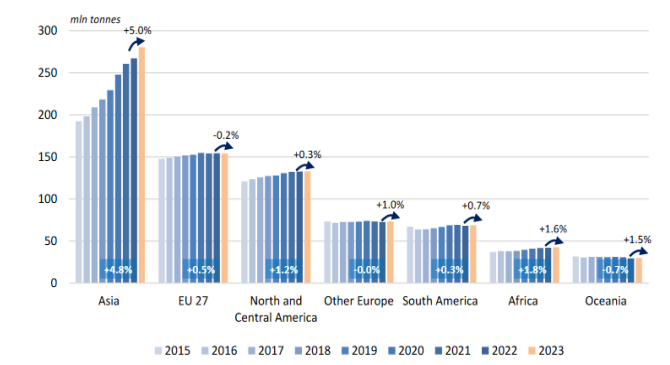
\includegraphics[width=0.8\textwidth]{media/ekon/image2}
	\caption*{Fig.3 - Major global milk producers in 2015-2023, million tons {[}6{]}}
\end{figure}

\begin{multicols}{2}
The dairy market is projected to undergo significant changes over the
next decade, influenced by various factors including consumption trends,
production dynamics, and global trade patterns. Key forecasts point to a
steady growth in global milk demand along with challenges such as price
fluctuations and resource costs. Global consumption of dairy products is
expected to grow due to population growth and increased health
awareness.

Production will be concentrated on fewer large farms, especially in
developed countries, leading to increased efficiency. The average farm
size is increasing and the number of dairy farms is decreasing,
reflecting the trend towards industrialization (Kozak \& Hryschenko,
2022) {[}7{]}. Although the dairy market shows promising growth, it is
important to consider the potential volatility and external factors that
may affect these forecasts. The relationship between demand, production
efficiency, and market risks will be critical in shaping the future
landscape of the dairy industry.

Several megatrends are influencing the development of the dairy market,
including changes in production and consumption, technological
advancements, and changing consumer preferences. All these factors
combine to shape the future of the dairy industry, highlighting both
opportunities and challenges.

Megatrends in dairy production and consumption:

- Geographic changes: there is a marked shift in dairy production from
the Global North to the Global South, driven by growing demand in
developing countries.

- Consumer preferences: the emergence of non-dairy alternatives is
changing the market dynamics and encouraging traditional dairy producers
to adapt (Bojovic \& McGregor, 2022) {[}8{]}.

- Technological advances: innovations in breeding, nutrition, and herd
management improve production efficiency and sustainability (Thornton,
2010) {[}9{]}.

- Market demand: the dairy sector is growing rapidly due to increased
consumer demand and improved supply chain (Fuller et al., 2015)
{[}10{]}.

- Environmental impact: The dairy industry is subjected to scrutiny of
environmental impact, so a balance between production and sustainability
is necessary (Bojovic \& McGregor, 2022).

Although the dairy market is poised for growth, it needs to overcome
challenges such as competition from plant-based products and the need to
adopt sustainable practices. The future remains uncertain due to
socio-economic factors and changing consumer values (Thornton, 2010).

One of the key indicators reflecting the efficiency of dairy farming is
productivity. In agricultural organizations of Kazakhstan, the
productivity of cows exceeded 5 thousand kg of milk with a fat content
of 3.8\%. This positive dynamics was the result of comprehensive
measures to develop dairy farming, including increasing the level of
production culture and improving the quality of fodder {[}11{]}.

The next most important indicator of dairy cattle breeding development
is the volume of marketable milk. The main growth of this indicator is
associated with the growth of milk yield in peasant/farmer farms and in
subsidiary farms of the population, although the level of average milk
yield is higher in agricultural organizations (Table 1).
\end{multicols}

{\bfseries Table 1 - The efficiency of milk and dairy products production by category of farms in Kazakhstan for 2022-2023}

%% \begin{longtable}[]{@{}
%%   >{\raggedright\arraybackslash}p{(\linewidth - 24\tabcolsep) * \real{0.1320}}
%%   >{\centering\arraybackslash}p{(\linewidth - 24\tabcolsep) * \real{0.0923}}
%%   >{\centering\arraybackslash}p{(\linewidth - 24\tabcolsep) * \real{0.0897}}
%%   >{\centering\arraybackslash}p{(\linewidth - 24\tabcolsep) * \real{0.0554}}
%%   >{\centering\arraybackslash}p{(\linewidth - 24\tabcolsep) * \real{0.0764}}
%%   >{\centering\arraybackslash}p{(\linewidth - 24\tabcolsep) * \real{0.0661}}
%%   >{\centering\arraybackslash}p{(\linewidth - 24\tabcolsep) * \real{0.0537}}
%%   >{\centering\arraybackslash}p{(\linewidth - 24\tabcolsep) * \real{0.0782}}
%%   >{\centering\arraybackslash}p{(\linewidth - 24\tabcolsep) * \real{0.0792}}
%%   >{\centering\arraybackslash}p{(\linewidth - 24\tabcolsep) * \real{0.0585}}
%%   >{\centering\arraybackslash}p{(\linewidth - 24\tabcolsep) * \real{0.0866}}
%%   >{\centering\arraybackslash}p{(\linewidth - 24\tabcolsep) * \real{0.0792}}
%%   >{\centering\arraybackslash}p{(\linewidth - 24\tabcolsep) * \real{0.0528}}@{}}
%% \toprule\noalign{}
%% \multirow{3}{=}{\begin{minipage}[b]{\linewidth}\raggedright
%% ~Indicato
%% \end{minipage}} &
%% \multicolumn{3}{>{\centering\arraybackslash}p{(\linewidth - 24\tabcolsep) * \real{0.2374} + 4\tabcolsep}}{%
%% \multirow{2}{=}{\begin{minipage}[b]{\linewidth}\centering
%% All categories of households
%% \end{minipage}}} &
%% \multicolumn{9}{>{\centering\arraybackslash}p{(\linewidth - 24\tabcolsep) * \real{0.6306} + 16\tabcolsep}@{}}{%
%% \begin{minipage}[b]{\linewidth}\centering
%% Including
%% \end{minipage}} \\
%% & & & &
%% \multicolumn{3}{>{\centering\arraybackslash}p{(\linewidth - 24\tabcolsep) * \real{0.1962} + 4\tabcolsep}}{%
%% \begin{minipage}[b]{\linewidth}\centering
%% agricultural enterprises
%% \end{minipage}} &
%% \multicolumn{3}{>{\centering\arraybackslash}p{(\linewidth - 24\tabcolsep) * \real{0.2159} + 4\tabcolsep}}{%
%% \begin{minipage}[b]{\linewidth}\centering
%% individual entrepreneurs and peasant or farm enterprises
%% \end{minipage}} &
%% \multicolumn{3}{>{\centering\arraybackslash}p{(\linewidth - 24\tabcolsep) * \real{0.2185} + 4\tabcolsep}@{}}{%
%% \begin{minipage}[b]{\linewidth}\centering
%% households of population
%% \end{minipage}} \\
%% & \begin{minipage}[b]{\linewidth}\centering
%% 2023
%% \end{minipage} & \begin{minipage}[b]{\linewidth}\centering
%% 2022
%% \end{minipage} & \begin{minipage}[b]{\linewidth}\centering
%% 2023 in \% to 2022
%% \end{minipage} & \begin{minipage}[b]{\linewidth}\centering
%% 2023
%% \end{minipage} & \begin{minipage}[b]{\linewidth}\centering
%% 2022
%% \end{minipage} & \begin{minipage}[b]{\linewidth}\centering
%% 2023 in \% to 2022
%% \end{minipage} & \begin{minipage}[b]{\linewidth}\centering
%% 2023
%% \end{minipage} & \begin{minipage}[b]{\linewidth}\centering
%% 2022
%% \end{minipage} & \begin{minipage}[b]{\linewidth}\centering
%% 2023 in \% to 2022
%% \end{minipage} & \begin{minipage}[b]{\linewidth}\centering
%% 2023
%% \end{minipage} & \begin{minipage}[b]{\linewidth}\centering
%% 2022
%% \end{minipage} & \begin{minipage}[b]{\linewidth}\centering
%% 2023 in \% to 2022
%% \end{minipage} \\
%% \midrule\noalign{}
%% \endhead
%% \bottomrule\noalign{}
%% \endlastfoot
%% Сattle & 8608852 & 8538050 & 100,8 & 864530 & 806691 & 107,2 & 3582638 &
%% 3373880 & 106,2 & 4161684 & 4357479 & 95,5 \\
%% of which are cows & 4765683 & 4462000 & 106,8 & 333142 & 317231 & 105 &
%% 2 037603 & 1881588 & 108,3 & 2394938 & 2263181 & 105,8 \\
%% Cow' s milk production, thousand tons & 6503,2 & 6320 &
%% 102,9 & 602,4 & 522,7 & 115,2 & 1427,6 & 1367 & 104,5 & 4473,1 & 4430,6
%% & 101 \\
%% Average milk yield per dairy cow, kg & 2~409 & 2 395 & 100,6 & 5~543 & 5
%% 128 & 108 & 1~849 & 1 860 & 99,4 & 2~459 & 2 459 & 100 \\
%% \multicolumn{13}{@{}>{\centering\arraybackslash}p{(\linewidth - 24\tabcolsep) * \real{1.0000} + 24\tabcolsep}@{}}{%
%% \emph{Note - compiled by the authors on the basis of the conducted
%% research {[}11{]}.}} \\
%% \end{longtable}

\begin{multicols}{2}
Prospective development of the raw milk market in Kazakhstan requires
attention to improving the material and technical base of dairy cattle
breeding. This is due to the slow introduction of innovative
technologies in this sector, which makes it one of the most labor- and
capital-intensive among livestock breeding areas. Despite the
mechanization of some labor-intensive processes, the level of labor
productivity remains low. For example, in foreign countries there are
35-40 cows per employee, while in Kazakhstan this indicator is only
13-16 cows. As a result, labor inputs for production of 1 centner of
milk on mechanized farms abroad are 0.6-0.6 person-hours, while in
Kazakhstan this indicator is 4 times higher and reaches 2.5-3.0
person-hours.

{\bfseries Conclusion.} Key factors negatively affecting the development of
the dairy subcomplex in Kazakhstan include: the low competitiveness of
products due to weak scientific and technical equipment, the
consequences of structural changes in the agro-industrial complex in the
1990s, which led to a reduction in milk production, and lower efficiency
of the industry, the dependence of the dairy subcomplex on climatic
conditions affecting the formation of the fodder base.

The Republic of Kazakhstan has developed state support measures, such as
the ``National Project for the Development of the Agro-Industrial
Complex of the Republic of Kazakhstan for 2021-2030''. The main
attention is paid to raw milk producers: subsidies are provided for
investment projects, short-term loans, construction of dairy farms, and
increasing the productivity of dairy cattle. However, milk processors
are left out of direct financial support, which creates an imbalance in
the development of the production and marketing chain {[}12, 13{]}.
Unlike the EU and the USA, where there are mechanisms of fair
distribution of income between producers of raw materials and,
processors and trade, in Kazakhstan there is no regulatory mechanism to
avoid price conflicts. This leads to the fact that raw material
producers and processors are forced to sell products below cost, and
small and medium-sized enterprises face pressure from network trade.

We offer the following recommendations for the development of the dairy
subcomplex of Kazakhstan, based on successful international practices,
including the following areas:

1. Introduction of carbon-neutral farms. In the EU countries, New Zealand
and Canada are actively developing projects of carbon-neutral
agriculture, based on technology that reduces greenhouse gas (methane)
emissions, and the creation of waste treatment systems. In Kazakhstan,
it is necessary to stimulate farms to install biogas plants that
convert livestock waste into energy, develop a support program for the
introduction of technologies to reduce emissions, through changing the
diet of cows or the use of special feed additives that reduce methane
emissions, the introduction of carbon subsidies for farmers who
modernize their farms to meet environmental standards.

2. Creating dairy innovation hubs. In the Netherlands and Denmark, there
are specialized hubs where farmers, researchers, and companies
cooperate to develop and test new technologies. In Kazakhstan, the
creation of such hubs is possible at agrarian universities and
research centers with the involvement of international experts and
private investors. In these hubs, farmers will be able to test new
technologies, and receive consultations on their implementation and
adaptation.

3. Development of contract farming. India, Brazil, and Kenya are actively
developing contract farming, where processing companies enter into
long-term contracts with farms, ensuring fixed prices for their
products. The introduction of contract farming in Kazakhstan will
allow processing companies, and retailers to provide farmers with
seeds, feed, and equipment in exchange for a commitment to supply milk
at fixed prices. This measure will be possible only based on a
developed legislative framework to protect the interests of both
parties.

4. Application of blockchain technology in supply chains. In the USA and
Australia, blockchain technologies are actively used for supply
transparency, tracing the origin of products and quality control. In
Kazakhstan, it is necessary to create a platform that integrates all
participants in the chain: farmers, processors, logistics companies
and retailers. The introduction of this technology in Kazakhstan will
help guarantee the quality and safety of products and increase
consumer confidence.

5. Development of digital markets for farmers. India and Kenya have
introduced digital platforms for farmers, allowing them to sell
directly to consumers and processors, bypassing intermediaries. The
creation of Kazakhstan' s digital platform for farmers,
where they can place offers to sell milk, fodder, or equipment, as
well as the development of a mobile application with the functions of
monitoring market prices and receiving a subsidy will reduce the
dependence of farmers on intermediaries and increase their income.

6. Transition to pasture-based livestock production. In New Zealand and
Australia, most of the milk is produced on pasture farms, which
reduces feed costs and improves milk quality. In Kazakhstan, the
implementation of this measure is possible based on pasture
modernization programs: their reclamation, planting of grasses
resistant to Kazakh climatic conditions, development of pasture
rotation systems to prevent land degradation, introduction of
subsidies for farmers switching to pasture-based animal husbandry.

7. Product diversification and development of niche markets. In the EU
countries, niche areas are successfully developing organic milk,
lactose-free products, and functional nutrition. In Kazakhstan, it is
necessary to develop measures to support producers of organic and
specialized dairy products through subsidies and grants, training of
farmers and processors of organic production standards, promotion of
niche products in foreign markets under the national brand.
The results of the implementation of these measures will reduce the
environmental load and increase the competitiveness of Kazakhstani
products in international markets, where environmental sustainability is
increasingly valued, accelerate the introduction of advanced
technologies and improve the interaction between science and practice,
reduce financial risks for farmers, sustainability of raw material
supplies for processors and increase price transparency, increase
confidence in Kazakhstani dairy products in international markets and
optimize internal processes, reduce dependence on dairy products, and
improve the quality of dairy products.

Thus, increasing the economic efficiency of the dairy subcomplex
requires a comprehensive approach, including reforms at the level of
individual economic entities and improvement of government policy.
Adaptation of advanced technologies and strategies to national
conditions will ensure the competitiveness of Kazakhstani products in
the world market and strengthen the country' s position
in the agro-industrial sector.
\end{multicols}

\begin{center}
{\bfseries References}
\end{center}

\begin{references}
1. Bartosz Mickiwicz, Katsiaryna Volkava Clobal Consumer Trends for
Sustainable Milk and Dairy Production// VUZF
Review.-2022.-Vol.7(2).-P.183-192. DOI 10.38188/2534-9228.22.2.9

2. Ob utverzhdenii nauchno obosnovannyh fiziologicheskih norm
potreblenija produktov pitanija //Prikaz Ministra
nacional' noj jekonomiki Respubliki Kazahstan ot 9
dekabrja 2016 goda № 503. Zaregistrirovan v Ministerstve justicii
Respubliki Kazahstan 13 janvarja 2017 goda № 14674. -
https://adilet.zan.kz/rus/docs/V1600014674 - Date of address:
02.01.2025. {[}in Russian{]}

3. Kazahstan obespechivaet sebja molochnymi produktami, bez ucheta
svezhego moloka, na 82,5\% - Economic Research Institute.
\url{https://dairynews.today/kz/news/kazakhstan-obespechivaet-sebya-molochnymi-produktami-bez-ucheta-svezhego-moloka-na-82-5-economic-res.html}-
Date of address: 02.01.2025.{[}in Russian{]}

4. Suraj, N.M. Mirovoj i otechestvennyj opyt v razvitii rynka moloka i
molochnyh produktov/ N.M.Suraj {[}i dr.{]}// Jekonomicheskie nauki.
2019. № 171. S.71--79. DOI 10.14451/1.171.71.{[}in Russian{]}

5. The World Dairy Situation Report 2023.
\url{https://milksa.co.za/sites/default/files/2024-01/2023\%20World\%20Dairy\%20Situation\%20Report.pdf}.
- Date of address: 02.01.2025.

6. FAO. Available at: URL: https://www.fao.org/statistics/en - Date of
address: 02.01.2025.

7. Kozak O., Grishhenko,O. Rinok moloka і molochnih produktіv: svіtovі
tendencії rozvitku ta perspektivi dlja Ukraїni. Herald of Khmelnytskyi
National University. Economic Sciences.-2022.- Т.308(4).- S.90-96. DOI
0.31891/2307-5740-2022-308-4-14 {[}in Ukrainian\}

8. Bojovic, M., \& McGregor, A. (2022). A review of megatrends in the
global dairy sector: what are the socioecological implications?//
Agriculture and Human.-2022.-Vol.40(3)

DOI 10.1007/s10460-022-10338-x

9. Philip, K., Thornton. (2010). Livestock production: recent trends,
future prospects. Phil Trans R Soc B//Philosophical
Transactions.-2010.-Vol.365(1554).-P.2853-2867

DOI 10.1098/RSTB.2010.0134

10. Frank, H., Fuller., Jikun, Huang., Hengyun, Ma., Scott, Rozelle. The
Rapid Rise of China' s Dairy Sector: Factors Behind the
Growth in Demand and Supply // American Journal of Agricultural
Economics.- 2005.- 38 p. DOI 10.22004/AG.ECON.18456

11. Bjuro nacional' noj statistiki RK.
https://stat.gov.kz/en/.- Date of address: 02.01.2025. {[}in Russian{]}

12. Nacional' nyj proekt po razvitiju agropromyshlennogo
kompleksa RK na 2021-2025 gody» (Postanovlenie
Pravitel' stva RK ot 12.10.2021 №732) Date of address:
02.01.2025. {[}in Russian{]}

13. «Koncepcija razvitija agropromyshlennogo kompleksa Respubliki
Kazahstan na 2021 - 2030 gody» (Postanovlenie
Pravitel' stva RK ot 30.12.2021 № 960) Date of address
02.01.2025. {[}in Russian{]}
\end{references}

\begin{authorinfo}
\emph{{\bfseries Information about the authors}}

Baiguzhinova A.- senior lecturer, Sarsen Amanzholov East Kazakhstan
University, Ust-Kamenogorsk, Kazakhstan e-mail:
\href{mailto:alma.b.78@mail.ru}{\nolinkurl{alma.b.78@mail.ru}};

Baidalinova A.- PhD, Acting Associate Professor, Department of
Management, Esil University, Astana, Kazakhstan, e-mail:
aynur.sultanovna@mail.ru;

Baigireeva Zh.- PhD, Acting Associate Professor, Department of
Management, Esil University, Astana, Kazakhstan, e-mail:
\href{mailto:zhanaruskaman@mail.ru}{\nolinkurl{zhanaruskaman@mail.ru}}

\emph{{\bfseries Сведения об авторах}}

Байгужинова А.Ж. -- сениор-лектор, Восточно-Казахстанский университет
имени С. Аманжолова, Усть-Каменогорск, Казахстан, e-mail:
\href{mailto:alma.b.78@mail.ru}{\nolinkurl{alma.b.78@mail.ru}};

Байдалинова А.С.-PhD, и.о. доцента кафедры «Менеджмент», Esil
University, Астана, Казахстан, e-mail:
\href{mailto:aynur.sultanovna@mail.ru}{\nolinkurl{aynur.sultanovna@mail.ru}};

Байгиреева Ж.З.- PhD, и.о. доцента кафедры «Менеджмент», Esil
University, Астана, Казахстан, e-mail:
\href{mailto:zhanaruskaman@mail.ru}{\nolinkurl{zhanaruskaman@mail.ru}}
\end{authorinfo}
